\documentclass[tp]{lcc}

% add latex preamble
% para la bibliografía se requiere biber y configurar texstudio

% Latex packages
\usepackage[utf8]{inputenc}
\usepackage[T1]{fontenc} % para copiar acentos en español del pdf y permite acentos en las notas
\usepackage[spanish]{babel}
\usepackage[per-mode = symbol]{siunitx} % para manejar las unidades
\usepackage{multimedia} % to add videos with \movie command
\usepackage{multirow}
\usepackage{graphicx}
\usepackage{xcolor}
\usepackage{amsmath} % bmatrix
\usepackage[makeroom]{cancel} % \cancel to cancel terms in math equations
\renewcommand{\CancelColor}{\color{red}} % set red color for \cancel command
\usepackage[caption=false]{subfig} % caption = false elimina la palabra "Figura" del caption
\usepackage{import} % para el comando import (se usa para pdf_tex)
\captionsetup[subfigure]{labelformat=empty} % remover el indice del caption de la subfigura
\usepackage{booktabs} % \toprule \midrule \bottomrule
\usepackage[backend=biber]{biblatex} % set biber to format references. Must configure Biber in Texstudio
\usepackage{csquotes} % to remove warning triggered by biblatex and babel
\usepackage{algorithm} % to put captions to the algorithmics environmets
\usepackage{algpseudocode} % to write algorithm
\usepackage{tikz} % to use tikz
\usetikzlibrary{fit} % to fit a node around other nodes in tikz
\usepackage[export]{adjustbox} % valign in subfloat
\usepackage{colortbl} % to paint cells in a table

% Color commands for annotations
\newcommand\TODO[1]{\textbf{\textcolor{red}{#1}}} %  TODO notes

% Graphic paths
\graphicspath{{./images/}}

% listings configuration for C code
\usepackage{listings} % code
\definecolor{commentgreen}{RGB}{2,112,10}
\definecolor{eminence}{RGB}{108,48,130}
\definecolor{weborange}{RGB}{255,165,0}
\definecolor{frenchplum}{RGB}{129,20,83}

\lstset{ % spanish characters for listings package
	inputencoding=latin1,
    columns=fullflexible,
	breaklines=true,
	tabsize=2,
	showstringspaces=false,
	basicstyle=\ttfamily,
	backgroundcolor=\color{lightgray}, % Choose background color
	literate={á}{{\'a}}1
	{ã}{{\~a}}1
	{é}{{\'e}}1
	{ó}{{\'o}}1
	{í}{{\'i}}1
	{ñ}{{\~n}}1
	{¡}{{!`}}1
	{¿}{{?`}}1
	{ú}{{\'u}}1
	{Í}{{\'I}}1
	{Ó}{{\'O}}1
    {-}{-}1
}

\lstdefinestyle{cpp}{ % spanish characters for listings package
    language=C++,
   	commentstyle=\color{commentgreen},
    keywordstyle=\color{eminence},
    stringstyle=\color{red},
    emph={int,char,double,float,unsigned,void,bool},
    emphstyle={\color{blue}}
}

\lstdefinestyle{bash}{ % spanish characters for listings package
	language=Bash
}

\lstdefinestyle{xml}{
	language=XML,
	morekeywords={encoding,xs:schema,xs:element,xs:complexType,xs:sequence,xs:attribute}
}

\lstdefinestyle{cmake}{
	language=make, % there is no cmake support in listings
}

\lstdefinestyle{python}{
    language=python,
}


%%%%% PARA QUE EN LAS TABLAS SE PUEDA PONER UN SALTO DE LINEA DENTRO DE UNA CELDA
\newcommand{\specialcell}[2][c]{%
    \begin{tiny}
        \begin{tabular}[#1]{@{}c@{}}#2\end{tabular}  
    \end{tiny}
}
%%%%%%%%%%%%%%%%%%%%%%%%%%%%%%%%%%%%%%%%%%%%%%%%%%%%%%%%%%%%%%%%%%%%%%%%

%%%%% PARA QUE LAS TABLAS TENGAN TODAS LAS COLUMNAS CENTRADAS Y DE IGUAL TAMAÑO
\usepackage{tabularx}
\renewcommand{\tabularxcolumn}[1]{>{\centering\arraybackslash}m{#1}}
%%%%%%%%%%%%%%%%%%%%%%%%%%%%%%%%%%%%%%%%%%%%%%%%%%%%%%%%%%%%%%%%%%%%%%%%



% add math preamble
\usepackage{amsmath}
\usepackage{amssymb}
\usepackage{amsopn}
\usepackage{mathtools}

% math
\renewcommand{\vec}[1]{\boldsymbol{\mathbf{#1}}}
\newcommand{\norm}[1]{\lVert#1\rVert}

% Declare arg max and arg min functionss
\DeclareMathOperator*{\argmax}{arg\,max}
\DeclareMathOperator*{\argmin}{arg\,min}

% Homogeneous decoration function
\newcommand{\homo}[1]{\dot{#1}}


% Declare projection as math function
\DeclareMathOperator{\proj}{proj}
\newcommand{\fromCoord}[2]{{#1}_\mathrm{#2}}
\newcommand{\toCoord}[2]{\prescript{\mathrm{#2}}{}{#1}}
\newcommand{\worldCoordSystem}{\mathrm{w}}
\newcommand{\bodyCoordSystem}{\mathrm{B}}
\newcommand{\cameraCoordSystem}{\mathrm{c}}
\newcommand{\point}{\vec{p}}
\newcommand{\worldPoint}{\toCoord{\point}{\worldCoordSystem}}
\newcommand{\imagePoint}{\vec{u}}
\newcommand{\cameraPoint}{\toCoord{\point}{\cameraCoordSystem}}
\newcommand{\homoWorldPoint}{\toCoord{\homo{\point}}{\worldCoordSystem}}
\newcommand{\homoImagePoint}{\homo{\imagePoint}}
\newcommand{\homoCameraPoint}{\toCoord{\homo{\point}}{\cameraCoordSystem}}
\newcommand{\measurement}{\vec{z}}
\newcommand{\prediction}{\hat{\vec{z}}}
\newcommand{\seMatrix}{\vec{\xi}}
\newcommand{\transform}[2]{\toCoord{\fromCoord{\seMatrix}{#2}}{#1}}
\newcommand{\pointCoord}[1]{\toCoord{\point}{#1}}
\newcommand{\rotation}{\vec{R}}
\newcommand{\rotationCoord}[2]{\toCoord{\fromCoord{\rotation}{#2}}{#1}}
\newcommand{\translation}{\vec{t}}
\newcommand{\translationCoord}[2]{\toCoord{\fromCoord{\translation}{#2}}{#1}}
\newcommand{\intrinsicMatrix}{\vec{K}}
\newcommand{\principalPoint}{\vec{c}}
\newcommand{\reprojectionError}{u}
\newcommand{\projectionMatrix}{\vec{P}}
\newcommand{\cameraCenter}{\vec{o}}
\newcommand{\essentialMatrix}{\vec{E}}
\newcommand{\inverse}[1]{{#1}^{-1}}

% Motion model
\newcommand{\position}{\vec{p}}
\newcommand{\orientationQuaternion}{\vec{q}}
\newcommand{\predictedPosition}{\hat{\vec{p}}}
\newcommand{\predictedOrientationQuaternion}{\hat{\vec{q}}}
\newcommand{\linearVelocity}{\vec{v}}
\newcommand{\angularVelocity}{\vec{\omega}}

\DeclareMathOperator{\slerpOp}{slerp}
\newcommand{\slerp}[1]{\slerpOp{\left( #1 \right)}}

% Map structure
\newcommand{\map}{M}
\newcommand{\keyframesSet}{K}
\newcommand{\mapPointsSet}{P}
\newcommand{\observedMapPoints}{O}
\newcommand{\covisibilityKeyframes}{CK}
\newcommand{\localMap}{local\_map}



% Bundle Adjutment
\newcommand{\update}{\vec{\delta}}
\newcommand{\incremental}{\hat{\update}}


% Loop Closure names

% scaled operators and letters to fancy view
\newcommand{\sminus}{\scalebox{0.5}[1.0]{$-$}}
\newcommand{\splus}{\scalebox{0.6}[0.6]{$+$}}
\newcommand{\curr}{c}
\newcommand{\sind}[1]{\scalebox{0.6}[0.6]{$#1$}}
\newcommand{\ind}[1]{\scalebox{0.7}[0.7]{$#1$}}

\newcommand{\keyframe}{\vec{K}}
\newcommand{\bowVector}{\vec{v}}
\newcommand{\lcError}{\vec{\Omega}}
\newcommand{\relativeTransformation}{\seMatrix}
\DeclareMathOperator{\interpolate}{interpolate}

\newcommand{\relativeMotion}{\vec{\delta}}
\newcommand{\groundTruth}[1]{{#1}^{*}}



% definición del operador rot()
\DeclareMathOperator{\rotationOp}{rot}
\newcommand{\getRotation}[1]{\rotationOp{\left( #1 \right)}}

\DeclareMathOperator{\translationOp}{trans}
\newcommand{\getTranslation}[1]{\translationOp{\left( #1 \right)}}









\codigo{R-521}
\materia{Robótica Móvil}
\titulo{Transformaciones}

\soluciones
\commentstrue


\usepackage{biblatex}
%\addbibresource{refs.bib}

\begin{document}
\maketitle

\section{Entrega}
Se deberá entregar un informe realizado en Lyx\footnote{\url{https://www.lyx.org/}} o latex con los ejercicios resueltos y explicando la solución según lo vea necesario para su comprensión. Para realizar gráficos se recomienda la utilización de la herramienta inkscape\footnote{\url{https://inkscape.org/}}. Para el código se debe proveer el link de un repositorio git junto con un archivo README.md con las instrucciones de ejecución.

\section{Ejercicios}
Esta práctica es para ponerse a punto con transformaciones.

\ejercicio Para el sistema de coordenadas canónico de un robot móvil (x: hacia adelante, y: hacia la izquierda, z: hacia arriba) dibujar y resolver matemáticamente el sistema de coordenadas resultante luego de aplicar las rotaciones dadas.

    \begin{figure}[!h]
    \centering
    \hspace{-4cm}
    \subfloat[(0,0,0)]
    {
        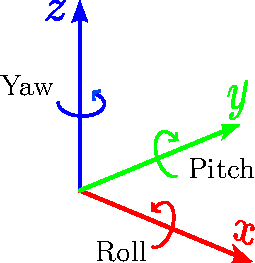
\includegraphics[width=0.2\columnwidth]{./images/roll_pitch_yaw.pdf}
    }
    \hspace{3cm}
    \subfloat[$R_{y}(\SI{90}{\degree})$]
    {
        
    }
    \hspace{3cm}
    \subfloat[$R_{x}(\SI{-90}{\degree})R_{y}(\SI{90}{\degree})$]
    {
    
    }
    \hspace{3cm}
    \subfloat[$R_{z}(\SI{180}{\degree})R_{x}(\SI{-90}{\degree})R_{y}(\SI{90}{\degree})$]{}
    \end{figure}

\ejercicio Dado el siguiente escenario,
\begin{itemize}
    \item un robot A que encuentra en la posición $(2,3)$ con orientación \SI{45}{\degree} en coordenadas del mundo
    \item un robot B que se encuentra en la posición $(1,1)$ con orientación \SI{-45}{\degree} en el sistema de coordenadas del robot A.
    \item un punto $\worldPoint1 = (1,5)$ en coordenadas del mundo.
    \item un punto $\toCoord{\point}{A}2 = (1,2)$ en coordenadas del robot A.
\end{itemize}
Resuelva:
\begin{enumerate}
    \item Dibuje los robots y las poses y todos los sistemas de coordenadas presentes
    \item ¿Cuáles son los coordenadas del punto $\point1$ en el sistema de coordenadas del robot A?
    \item ¿Cuáles son los coordenadas del punto $\point2$ en el sistema de coordenadas del robot B?
    \item ¿Cuál es la pose (posición y orientación) del robot B en coordenadas del Mundo?
\end{enumerate}

\ejercicio Data la pose del robot (Body) en el mundo: $\transform{W}{B}$. Si se tiene el camino (conjunto de poses $\transform{C_{0}}{C_{i}}$ con $i = 1 \dots n$) realizado por la cámara $C$ (montada sobre el robot) en el marco de coordenadas de la cámara inicial $C_{0}$. Sabiendo la transformación $\transform{B}{C}$, 
\begin{itemize}
	\item ¿Qué procedimiento hay que realizar para obtener el camino realizado por la cámara en el sistema de coordenadas del mundo?.
	\item ¿Qué procedimiento hay que realizar para obtener el camino realizado por el robot (Body) en el sistema de coordenadas del mundo?
    \item Realizar un gráfico ilustrativo donde se visualicen los sistemas de coordenadas, las transformaciones y los caminos realizados por el robot y la cámara.
\end{itemize}


\ejercicio Para este ejercicio utilizaremos el dataset EuRoc\footnote{\url{https://projects.asl.ethz.ch/datasets/kmavvisualinertialdatasets}}.

Descargue el archivo \emph{ground-truth} (trayectoria real realizada por el robot) localizado \url{ http://robotics.ethz.ch/~asl-datasets/ijrr_euroc_mav_dataset/machine_hall/MH_01_easy/MH_01_easy.zip}.

\begin{nota}
	Para la descarga se recomienda utilizar el programa \lstinline{aria2c} con los parámetros: \lstinline{aria2c -s N -x N <URL>}, con \lstinline{N} la cantidad de cores en su computadora.
\end{nota}

\begin{enumerate}
    \item El \emph{ground-truth} se encuentra en coordenadas de la IMU (Body). Se pide crear un script en python que dada la trayectoría ground-truth (timestamp, x, y, z, qw, qx, qy, qz) (primeras 8 columnas del archivo \lstinline{MH_01/state_groundtruth_estimate0.csv}) genere el ground-truth pero que este esté dado en el sistema de coordenadas de la cámara inicial. Para esto deberá utilizar las transformaciones provistas en el dataset.
    
    \item Modifique el script para que el timestamp del nuevo \emph{ground-truth} este en segundos con precisión de nanosegundos. Agregar las primeras 5 filas del ground-truth resultante y las del original del dataset al informe.
    
    \item Modifique el script para que genere una imagen con ambos \emph{ground-truth} (el camino de la IMU y el camino de la cámara). Aplique las transformaciones necesaria para que ambos caminos esten en el sisma de coordenadas del ground-truth original. Agregar la imagen al informe.
\end{enumerate}

\begin{nota}
	Para graficar en Python se recomienda utilizar la librería matplotlib\footnote{\url{https://matplotlib.org/}}. Para trabajar con transformaciones en Python se recomienda utilizar la librería: transforms3d\footnote{\url{https://github.com/matthew-brett/transforms3d}}
\end{nota}




\end{document}
